\section{Mogan STEM: A WYSIWYG Structured Editor}
\label{sec:mogan}

Since last year, the maintainers of the Chinese TeXmacs community have developed Mogan STEM~\cite{moganstem2025} and a commercial version, Liii STEM~\cite{liiistem2025}, based on GNU TeXmacs. Currently, Mogan STEM and TeXmacs stand as the world's only WYSIWYG structured editors. Table~\ref{tab:mogan-vs-other} compares Mogan STEM with several other editors currently available on the market.

\begin{table}[htbp]
\centering
\caption{Comparison between Mogan STEM and alternative editors}
\label{tab:mogan-vs-other}
\begin{tabular}{lcccc}
\toprule
\textbf{Editor} & \textbf{WYSIWYG} & \textbf{Structured} & \textbf{Unicode Support} & \textbf{\TeX{} Compatibility} \\
\midrule
\textbf{Mogan STEM} & Yes & Yes & Yes & Partial \\
\textbf{TeXmacs} & Yes & Yes & Partial & Partial \\
\textbf{TeX/LaTeX} & No & Yes & Partial & Full \\
\textbf{Word} & Yes & No & Partial & Incompatible \\
\textbf{LyX} & Partial & Yes & Partial & Full \\
\textbf{Typst} & No & Yes & Yes & Partial \\
\bottomrule
\end{tabular}
\end{table}

The core technical challenge in achieving the WYSIWYG capability of Mogan STEM lies in the representation and rendering of mathematical formulas. Unlike \TeX{}, which represents formulas through layout-oriented markup in the form of typesetting instructions, Mogan STEM adopts a tree-based, functional representation for both mathematical formulas and the document structure itself. The following discussion evaluates this mechanism with specific examples.

Mogan STEM is a WYSIWYG structured editor designed to address the limitations of \LaTeX{} while maintaining its strengths in scientific typesetting~\cite{moganstem2025, liiistem2025}. The key innovations of Mogan STEM include:

\subsection{Tree-Structured Formulas and Document Structure}
\label{sec:tree-struc-on-mogan}

Unlike \LaTeX{}'s compilation model, which centers on linear text and macro expansion, \TeX{}macs features an explicit tree-based document structure designed from the outset. Document components---such as chapters, formulas, citations, and typesetting elements---exist as structured nodes, rather than being implicitly embedded within macro calls or token streams. This architectural distinction directly impacts citation updates, compilation efficiency, and the interactive user experience.

Unlike \LaTeX{}'s linear macro-based representation, Mogan STEM represents documents as structured trees. This enables precise semantic understanding and manipulation of document elements.

A fraction serves as a primary example of this difference. In \TeX{}, a fraction is represented as \verb|\frac{1}{2}|; internally, the compiler processes \verb|\frac|, \verb|{1}|, and \verb|{2}| serially. In Mogan STEM, however, the fraction is represented at the underlying layer as the Scheme code \verb|(frac "1" "2")|.\footnote{Note that Mogan STEM is \textbf{WYSIWYG}; therefore, when inputting $\frac{1}{2}$, the user does not type \texttt{(frac 1 2)}, but instead presses \keys{Alt+f} to input it visually!} This forms a tree structure, as illustrated in Figure~\ref{fig:frac-tree}.


\begin{figure}[htbp]
\centering
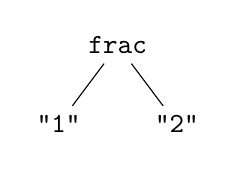
\begin{tikzpicture}[
    level 1/.style={sibling distance=15mm, level distance=10mm},
    every node/.style={align=center}
]
\node {\texttt{frac}}
    child {node {\texttt{"1"}}}
    child {node {\texttt{"2"}}};
\end{tikzpicture}
\caption{The Tree Structure of Mogan Formulas}
\label{fig:frac-tree}
\end{figure}

Figure~\ref{fig:frac-tree} illustrates how mathematical expressions are represented as trees in Mogan STEM. Each node has a specific type and contains its children in a well-defined structure. This representation enables:

\begin{itemize}
    \item Precise cursor positioning and navigation
    \item Structural selection and manipulation
    \item Semantic-aware editing operations
\end{itemize}

\begin{equation}
\label{eq:tree-struc}
\text{Tree}(f) = \begin{cases}
    (\text{leaf}, v) & \text{if } f \text{ is atomic} \\
    (\text{op}, [\text{Tree}(c_1), \ldots, \text{Tree}(c_n)]) & \text{otherwise}
\end{cases}
\end{equation}

Equation~\ref{eq:tree-struc} shows the recursive definition of the tree structure for formulas. Figure~\ref{fig:tree-representation} shows a tree representation of a mathematical expression.

\begin{figure}[htbp]
\centering
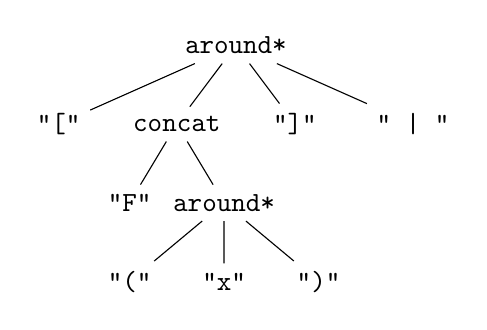
\begin{tikzpicture}[
    level 1/.style={sibling distance=15mm, level distance=10mm},
    level 2/.style={sibling distance=12mm, level distance=10mm},
    level 3/.style={sibling distance=12mm, level distance=10mm},
    every node/.style={align=center}
]
\node {\texttt{around*}}
    child {node {\texttt{"["}}}
    child {node {\texttt{concat}}
        child {node {\texttt{"F"}}}
        child {node {\texttt{around*}}
            child {node {\texttt{"("}}}
            child {node {\texttt{"x"}}}
            child {node {\texttt{")"}}}
        }
    }
    child {node {\texttt{"]"}}}
    child {node {\texttt{" | "}}};
\end{tikzpicture}
\caption{Tree representation of $ [F (x)] |$}
\label{fig:tree-representation}
\end{figure}

Unlike \TeX{}, this tree structure exists at the rendering level, not the syntax level. In fact, many long-time users of Mogan and \TeX{}macs cannot write a single line of Scheme code! This rendering-level tree structure offers two distinct advantages:

\begin{enumerate}
    \item \textbf{Local Scoping of Input Errors:}
    \begin{itemize}
        \item Errors do not cause the entire document to fail rendering (a major drawback of \LaTeX{}).
        \item Local edits do not trigger global layout instability (a major drawback of MS Word).
    \end{itemize}
    
    \item \textbf{Parallel Processing:} The CPU renders data in parallel rather than serially, which significantly accelerates rendering speed.
\end{enumerate}

Consider the following mathematical expression:
\begin{equation}
\int_{a}^{b} f(x) \mathrm{d}x = \left[ F(x) \right] \big|_{a}^{b}
\label{eq:integral-example}
\end{equation}

Its Scheme representation is as follows:
\begin{lstlisting}[caption={Scheme representation of integral expression},label={lst:scheme-integral}]
(math (concat (big "int") (rsub "a") (rsup "b")
       "f" (around* "(" "x" ")") "d" "x" "="
       (around* "<nobracket>" (around* "["
         (concat "F" (around* "(" "x" ")")) "]") "|")
       (rsub "a") (rsup "b")))
\end{lstlisting}

Note that the segment $\left[ F(x) \right] |$ is managed via the tree structure. Consequently, even if a user omits a parenthesis or two, this omission does not negatively affect the rendering of the entire mathematical expression in Mogan.

Figure~\ref{fig:double-line} illustrates image insertion between lines, and Figure~\ref{fig:multiline-mogan} shows Mogan's multi-line data structure.

\begin{figure}[htbp]
\centering
\includegraphics[width=0.3\textwidth]{figure/double-line.png}
\caption{Image insertion between lines}
\label{fig:double-line}
\end{figure}

\begin{figure}[htbp]
\centering
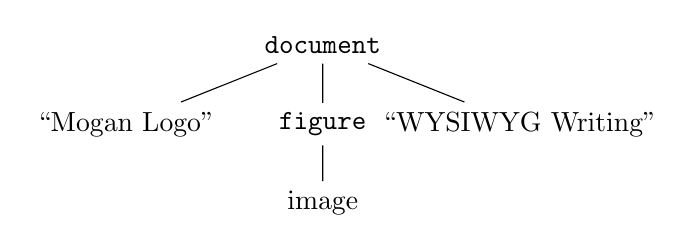
\begin{tikzpicture}[
    level 1/.style={sibling distance=25mm, level distance=10mm},
    level 2/.style={sibling distance=25mm, level distance=10mm},
    every node/.style={align=center}
]
\node {\texttt{document}}
    child {node {``Mogan Logo''}}
    child {node {\texttt{figure}}
        child {node {image}}
    }
    child {node {``WYSIWYG Writing''}};
\end{tikzpicture}
\caption{Mogan's multi-line data structure}
\label{fig:multiline-mogan}
\end{figure}

Let's look at another example. For a two-line layout like Figure~\ref{fig:double-line}, the Scheme representation is:
\begin{lstlisting}
(document "Mogan Logo" "(figure )" (itemize (document (concat (item) "WYSIWYG Writing") "")))
\end{lstlisting}

\subsection{Functional Symbol Representation}

Mogan STEM uses a functional representation for symbols and operators. This provides a clean, compositional semantics for document elements. For example, a fraction is represented as:

\begin{equation}
\label{eq:braket}
\text{frac}(a, b) \mapsto \frac{a}{b}
\end{equation}

This functional approach contrasts with \LaTeX{}'s macro-based approach, where \verb|\frac{a}{b}| relies on positional arguments and implicit grouping.

\subsection{Fast Reference Rendering}

Cross-references in Mogan STEM are maintained as bidirectional links in the document tree. When a label is updated, all references to it are automatically updated without requiring a full recompilation. This provides immediate visual feedback and eliminates the need for multi-pass compilation.

\subsection{On-demand plugin loading}

Mogan STEM's architecture supports on-demand loading of features and document types. Unlike \LaTeX{}, where the entire distribution must be installed upfront, Mogan loads only the components needed for the current document. This significantly reduces installation size and startup time.
